\chapter{Interpretations and implications of scaling laws}
\label{chap:scaling_implications}

\begin{flushright}{\slshape    
There are no facts, only interpretations.} \\ \medskip
--- Friedrich Nietzsche
\end{flushright}



\bigskip

Although allometric scaling relationships are a powerful tool to explore the
behaviour of cities, there are several continuing controversies in the
literature. First, about their interpretation: do these relationships say
something about cities and the processes they host, or cities as they relate to
one another in a system of cities? Second, recent
studies~\cite{Arcaute:2014,Louf:2014_mobility,Cottineau:2015} have shown that
the measured exponents are very sensitive to the way cities are defined. What
does it imply for the study of these scalings and, more generally, cities? 



\section{What scaling laws tell us about cities}

Scaling laws are, in essence, cross-sectionnal
studies of cities. As opposed to dynamical studies where one would follow the
evolution of individual cities over time, scaling laws tells us about the behaviour
of an \emph{ensemble} of cities at a give point in time. Throughout
Chapters~\ref{chap:scaling_introduction} and~\ref{chap:scaling_model}, we have
implicitely assumed that scaling laws are the signature of phenomena occuring at
the intra-urban level. This assumption, we call \emph{evolution interpretation},
is however not completely obvious. 

Maybe the easiest way to understand the issues posed by this interpretation is
through the comparison with Biology, where allometric scaling laws are also
widely used. The interpretation of allometric scaling laws in Biology is
straightforward, because the compared organisms are independent. Consider, for
instance, the scaling of the metabolic rate of animals with their body
mass~\cite{West:1997,Banavar:1999}. The mass of a given elephant at a point in
time $t$ is not correlated to the mass of any other living creature in the
world. Therefore, the scaling relationship can only be understood as resulting
from the existence  of similar processes in the growth of these different
animals.  Cities are different. They are part of a bigger system -- the system
of cities -- and interact constantly with one another. People change residence,
companies relocate, goods are shipped and money is transfered. Therefore, as
argued by Denise Pumain~\cite{Pumain:2012}, scaling laws can also be construed
as reflecting the redistribution processes within this system of cities. We call
this the \emph{differentiation interpretation}.

\subsection{The evolution interpretation}
\label{sub:the_evolution_interpretation}

The evolution interpretation (Figure~\ref{fig:evolution_interpretation}) has
been widely adopted in the scaling literature~\cite{Bettencourt:2007,
Bettencourt:2013,Louf:2014_scaling} without ever being clearly stated, let alone
justified. It is based on two assumptions. The first assumption is that cities in the dataset
are different realisations of the same system. Thus, as stated in
Chapter~\ref{chap:scaling_introduction}, looking at the scaling of various
quantities with population size is a way to probe the system's internal
processes.

\begin{figure}[!h]
    \centering
    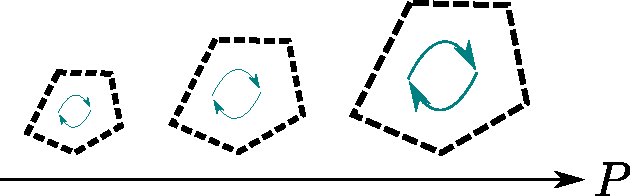
\includegraphics[width=\textwidth]{gfx/chapter-scaling/evolution-interpretation.pdf}
    \caption{{\bf Evolution interpretation.} In this interpretation we consider
    that cities are different realisations of the same system. The intra-urban
processes -- and the way they respond to population changes -- are responsible for the non-linear scaling of the different
quantities.\label{fig:evolution_interpretation}}
\end{figure}

The second assumption has to do with the time scales over which the different
processes occur. Indeed, if the processes responsible for the change in the
value of the quantity $Y$ being studied occur on timescales significantly larger
than the timescale over which the population size changes, we cannot be sure the
exponent value actually reflects the internal processes at the time we measure
it.  For instance, an abrupt increase in population size is not likely to be
immediately reflected in the length of streets, while the evolution of the total
commuted length will be almost instantaneous. In practice, the rate of population change in cities is small enough for the
processes to follow, or the amplitude small enough for the induced error to be
insignificant. Hence the observed stability in the value of some exponents.

The previous discussion has several important consequences. First, it hints at
the difficulty to intepret the values of the observed deviations to scaling
laws~\cite{Bettencourt:2010a}. It is indeed difficult to assess to what extent
deviations account for a real over- or under-performance of the city compared to
the other cities, or for the time it takes for the studied quantity to react to
population changes.  Worse, the delayed adjustment to population changes
introduces an irreducible uncertainty in the numerical values of the exponents
themselves. Thus, the real error on the measured value of the exponent is very
likely larger than what is usually indicated by the statistical error bars.
Unfortunately, we cannot get a better estimate of the error until we understand
in details the mechanisms responsible for the time evolution of the corresponding
quantities. Until then, we should focus on (1) trying to understand the
qualitative behaviour, more than the exact numerical value of the exponents (2)
be wary of interpreting exponent values that are close to 1 (typically between $0.90$ and
$1.10$); in the absence of an alternative mechanistic explanation, the linear
relationship has to be favoured due to its simplicity.


\subsection{The differentiation interpretation}
\label{sub:the_differentiation_interpretation}

As Denise Pumain judiciously claims~\cite{Pumain:2006,Pumain:2012}, the evolution
interpretation is not the only possible interpretation for scaling laws. In some
cases and the mechanisms responsible for scaling relationships should be sought
after in the hierarchical organisation of cities and their interactions.\\

\begin{figure}[!h]
    \centering
    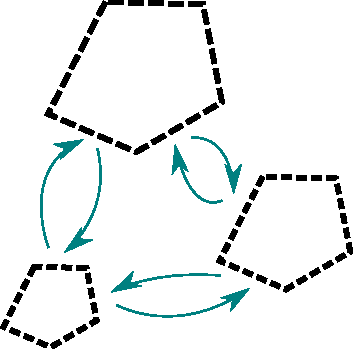
\includegraphics[width=0.5\textwidth]{gfx/chapter-scaling/system-interpretation.pdf}
    \caption{{\bf Differentiation interpretation.} In this interpretation, we
    consider that the redistribution processes occuring within systems of cities
are reponsible for the non-linear scaling of quantities with city size in this
system.\label{fig:label_fig}}
\end{figure}

We briefly mentioned in Chapter~\ref{chap:scaling_model} that allometric scaling relationships
could only be obtained when considering cities that belong to the same system of
cities. The fact that we observe scalings when taking a single country into
account, and a cloud of points when mixing two different countries, is a
signature of the integration of cities into systems of cities. It is
not clear at the moment what mechanisms are reponsible for the
coherence that permits the existence of scaling at the system level. But
clearly, the fact that cities are tightly connected through
the flow of commodities, populations, information and funds must be a key
factor.\\

Now, the same connections may be responsible for the scaling relationships
themselves, and the value of the exponent. As an example, Pumain et
al.~\cite{Pumain:2006} study the scaling of the number of employees from
different economic sectors in France with population size (see also
Chapter~\ref{chap:scaling_introduction}). They find that the number of employees
in innovative sectors (such as research and development) scales superlinearly
with population size, while the number of employees in mature economic sector
(such as the manufacture of food products) scales sublinearly with population
size. Using historical data, they further show that the scaling behaviour of
some activities has significantly changed over time: the exponent of
manufacturing activities has continuously decreased since $1960$, while that of
research and developement has continuously increased. This could be explained,
they claim, by the hierarchical diffusion of innovations in systems of cities.
Innovative activities first appear in large cities, entailing a larger
proportion of the active population working in these sectors than in smaller
cities, thus a superlinear scaling.  Over time, the innovations progressively
diffuse through the system of cities, the proportions are equilibrated and the
value of the scaling exponent decreases.

Although the mechanism is plausible, the current issue with this interpretation
is the lack of predictive model that explains the values of the various
exponents. 


\subsection{Cities, or systems of cities?}
\label{sub:cities_or_systems_of_cities_}

So, are scaling relationships properties of cities, or of systems of cities?
Probably both. The above discussion is very general, and the origin of scalings
should be evaluated on a case-by-case basis. The scaling of some quantities,
such as the total quantity of CO\textsubscript{2} emitted or the total length of
roads are undoubtedly due to intra-urban processes (at least as long as the
explanation presented in Chapter~\ref{chap:scaling_model} holds). Indeed, the
total length of roads in Los Angeles only depends on what happens in Los
Angeles. Others, such as the linear
scaling of total income, are probably due to the interactions of cities within
the same system of cities. However, it is impossible to discriminate between
both interpretations on a purely empirical basis. Ultimately, we need models that are
able to reproduce at least the qualitative scaling behaviour. Plausible
narratives are not enough.


\section{What cities?}
\label{sec:what_cities_}

As we have argued up to this point, scaling relations are a signature
of various processes governing the phenomenon under study, especially when the exponent
$\beta$ is not what is naively expected~\cite{Barenblatt:1996}. However, as more and more scaling
relationships are being reported in the literature, it becomes less and less clear what we really
learn from these empirical findings. Mechanistic insights about these scalings are usually
nonexistent, often leading to misguided interpretations.


A striking example of the fallacies which hinder the interpretation and
application of scaling is given by different studies on $CO_2$ emissions due to
transportation~\cite{Fragkias:2013,Glaeser:2010,Oliveira:2014,Rybski:2013}. The
topic is particularly timely: pollution peaks occur in large cities worldwide
with a seemingly increasing frequency, and are suspected to be the source of
serious health problems~\cite{Bernstein:2004}. Glaeser and
Kahn~\cite{Glaeser:2010}, Rybski et al~\cite{Rybski:2013}, Fragkias et
al~\cite{Fragkias:2013}, and Oliveira et al~\cite{Oliveira:2014} are interested
in how $CO_2$ emissions scale with the population size of cities. The question
they ask is simple: Are larger cities greener---in the sense that there are
fewer emissions per capita for larger cities---or smoggier? Surprisingly, these
different studies reach contradictory conclusions. We identify here two main
sources of error which originate in the lack of understanding of the mechanisms
governing the phenomenon.

The first error concerns the estimation of the quantity $Q_{CO_2}$ of $CO_2$ emissions due to
transportation. In the absence of direct measures, Glaeser and Kahn~\cite{Glaeser:2010} have chosen
to use estimations of $Q_{CO_2}$ based on the total distance traveled by commuters. This is in fact
incorrect, and in heavily congested urban areas the relevant quantity is the total time spent
in traffic~\cite{Louf:2014_mobility}. Using distance leads to a serious underestimation of
$CO_2$ emissions: the effects of congestion are indeed strongly nonlinear, and the time spent
in traffic jams is not proportional to the traveled distance. As a matter of fact, commuting
distance and time scale differently with population size, and the time spent commuting and
$CO_2$ emissions scale with the same exponent~\cite{Louf:2014_mobility}.

The second, subtler, issue lies in the definition of the city itself, and over
which geographical area the quantities $Q_{CO_2}$ and $P$ should be aggregated.
There is currently great confusion in the literature about how cities should be
defined, and scientists, let alone the various statistical agencies in the
world, have not yet reached a consensus. For instance, the US Census Bureau
defines two types of cities for statistical purposes
(see Figure~\ref{fig:two_definitions} for an illustration on the city of Minneapolis).
First, the Urban Areas are defined as a set of contiguous high-density areal
units with a threshold on the total population (morphological definition). The Metropolitan Statistical
Areas, on the other hand, include core Urban Areas, and the areal units that
sends more than a given percentage of its working population to work in the
core (functional definition).

\begin{figure}
    \centering
    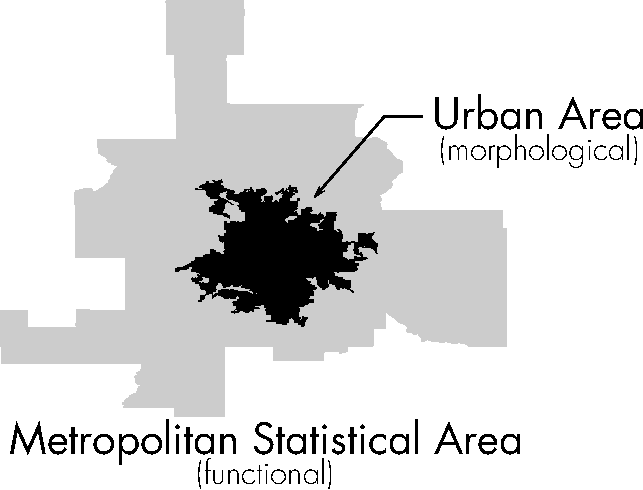
\includegraphics[width=\textwidth]{gfx/chapter-scaling/city_definition.pdf}
    \caption{{\bf City definitions in the US.} The Minneapolis Urban Area (in
    black) is defined by the Census Bureau as contiguous block groups with at
least $1000$ inhabitants per square mile. The Minneapolis-St. Paul Metropolitan
Statistical Area (in grey) is defined as the counties containing the urban area
as well as any adjacent county that have a high degree of integration with the
core, as measured with commuting flows.\label{fig:two_definitions}}
\end{figure}


This is a crucial issue as scaling exponents are very sensitive to the
way city boundaries are delineated~\cite{Arcaute:2014}.  $CO_2$ emissions are no exception:
aggregating over Urban Areas or Metropolitan Statistical Areas entails radically
different behaviours (see Figure~\ref{fig:lost}). For the US, using the
definition of urban areas provided by the Census Bureau
(\url{http://www.census.org}), one finds that $CO_2$ emissions per capita
sharply increase with population size, implying that larger cities are less
green. Using the definition of metropolitan statistical areas, also provided by
the Census Bureau, one finds that $CO_2$ emissions per capita decrease slightly
with population size, implying that larger cities are greener.\\

\begin{figure}[!h]
	\centering
	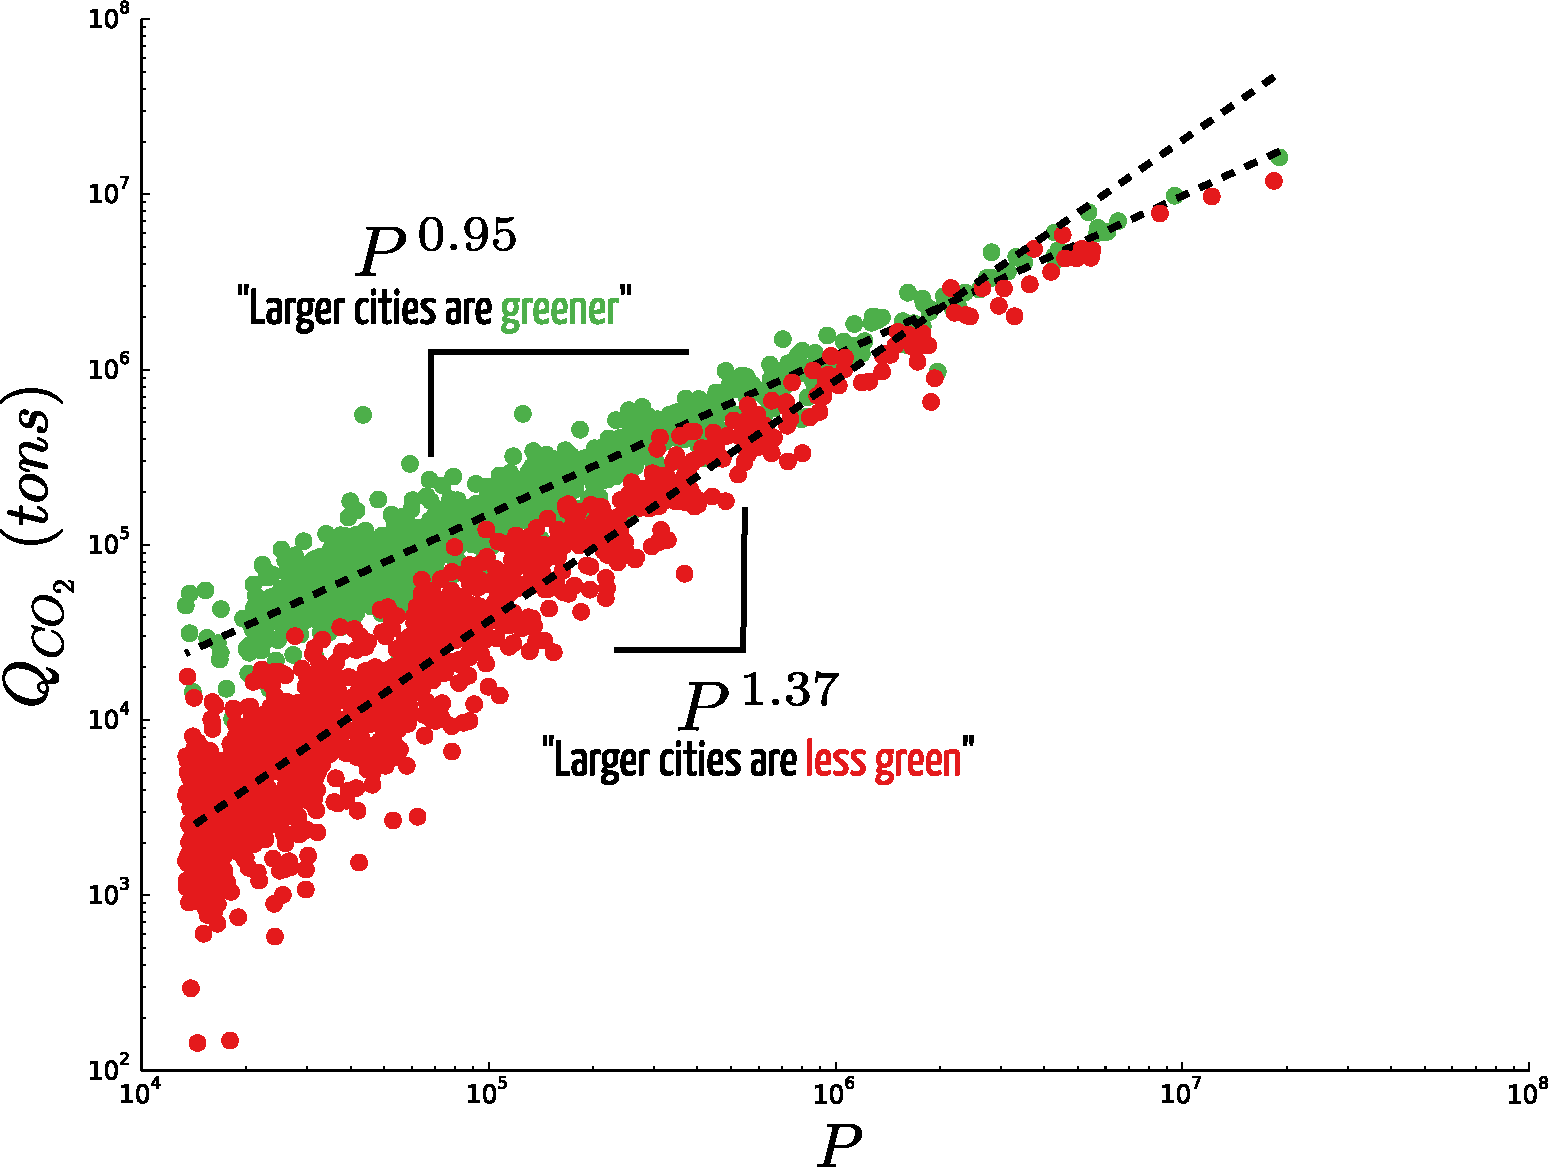
\includegraphics[width=\textwidth]{gfx/chapter-scaling/lost_smog.pdf}
	\caption{ {\bf Are larger cities greener or smoggier?} Scaling of transport-related $CO_2$
emissions with the population size for US cities from the same dataset but at different aggregation
levels. In red, the aggregation is done at the level of urban areas and in green for combined statistical
areas. Depending on the definition of the city, the scaling exponents are qualitatively different, leading
to two opposite conclusions. Data on $CO_2$ emissions were obtained from the Vulcan Project (\url{http://
vulcan.project.asu.ed}) (see~\cite{Fragkias:2013,Oliveira:2014}). Data on the population of urban areas and
metropolitan statistical areas were obtained from the Census Bureau
(\protect\url{http://www.census.org}). \label{fig:lost}}
\end{figure}


Faced with these two opposite results, what should one conclude? Our point is that, in
the absence of a convincing model that accounts for these differences and how they arise,
nothing. Scaling relationships, and more generally data analysis, have an important role
to play in the rising new science of cities. But, as the previous discussion
illustrates (as well as the discussion in Chapter~\ref{chap:methodology}), it is
dangerous to interpret empirical results without any mechanistic insight. Conclusions cannot
safely be drawn from data analysis alone.\\

Does it mean that we should throw away scaling relationships altogether, as
suggested by Arcaute et al.~\cite{Arcaute:2014}? No, this would be tackling the
problem from the wrong end. Scaling relationships are the signature of processes
occuring at the system (city or system of cities) level. The issue encountered
here is that the system we study is not properly defined. We don't really know
what cities we are talking about! 

Cities are doubtlessly a real pattern. Yet, the way we unveil this pattern with
empirical data is, at best, imprecise. It is not based on a theoretical
understanding of what cities are. As a result, we cannot fully make sense of the
exponents found in empirical data. We therefore believe that future research in
this area should focus on

\begin{itemize}
    \item Understanding the basic object we are working on, cities. How they 
        should be defined, on what theoretical grounds.
    \item Accounting for the different qualitative behaviours of scaling
        exponents when different definitions are used.
\end{itemize}

Indeed, as long as we do not \emph{know} what system we should be probing, it is
not quite clear what our results mean. As long as we do not \emph{understand}
why values of exponents are different when the city definition changes, we
cannot draw reasonable conclusions.\\

The last years have seen many scholars coming forward with policy advice based
on empirical scaling relationships. It should now be clear that, given the
current state of knowledge, it is a risky game. Indeed, let us consider the
above CO\textsubscript{2} example: what should one do to curb CO2 emissions?
Favour the growth of large urban areas or the repartition of population in less
populated cities?  Both can be argued by considering data analysis alone. It
should therefore be obvious that, until they have a satisfactory understanding
of the mechanisms responsible for the observed behaviours, scientists should
refrain from giving policy advice that might have unforeseen, disastrous
consequences. If they choose to do so anyway, policy makers should be wary about
what is, at best, a shot in the dark


\section{Conclusion and perspective}
\label{sec:conclusion_and_perspective}

Scaling laws are useful tool to probe the internals of cities, but they are not
everything. They provide an extraordinarily easy way to explore the properties
of urban systems: the amount of data required is minimal, the statistical treatment
trivial. Allometric scaling is thus useful to declutter the field of investigation, help clear
a couple of paths, and establish a large-scale understanding of the system. But
this is done at the expense of an extensive coverage of the underlying
phenomena. Scalings can be seen as a gateway to the study of cities, but they
cannot be the study itself.

Furthermore, there are pressing issues that need to be solved if we want to make
sense of these empirical results. First, we need to question the definition of
cities, and understand what systems exactly we are studying. Second, measuring
exponents is not enough, and we need to understand the main processes that are
responsible for the measured values. This is what we have tried to do in the
previous chapter.
